\chapter{\label{cap:3}Marco Metodol\'{o}gico}

	\section{Metodolog\'{i}a Investigaci\'{o}n-Acci\'{o}n}
	\cite{Baskerville} define la Investigaci\'{o}n-Acci\'{o}n como un m\'{e}todo de investigaci\'{o}n que a finales de la d\'{e}cada de los 90 empez\'{o} a crecer en popularidad, para el uso en investigaciones acad\'{e}micas de sistemas de informaci\'{o}n. Este m\'{e}todo produce resultados de investigaci\'{o}n altamente relevantes, debido a que se fundamenta en la acci\'{o}n pr\'{a}ctica, dirigida a resolver un problema mientras se informa cuidadosamente sobre la teor\'{i}a.

	Esta metodolog\'{i}a tiene una doble finalidad: generar un beneficio al cliente de la investigaci\'{o}n y al mismo tiempo, generar conocimiento de investigaci\'{o}n relevante. Por lo tanto, es una forma de investigar de car\'{a}cter colaborativo que busca unir teor\'{i}a y la pr\'{a}ctica entre investigadores y practicantes, mediante un proceso de naturaleza c\'{i}clica.

	La representaci\'{o}n m\'{a}s habitual de la Investigaci\'{o}n-Acci\'{o}n es la descrita por \cite{Baskerville}, en forma de cinco fases que conforman un ciclo, las cuales se describen en la Figura 1.

\FloatBarrier %you shall not pass table!!
\vline
	\begin{figure}
		\centering
		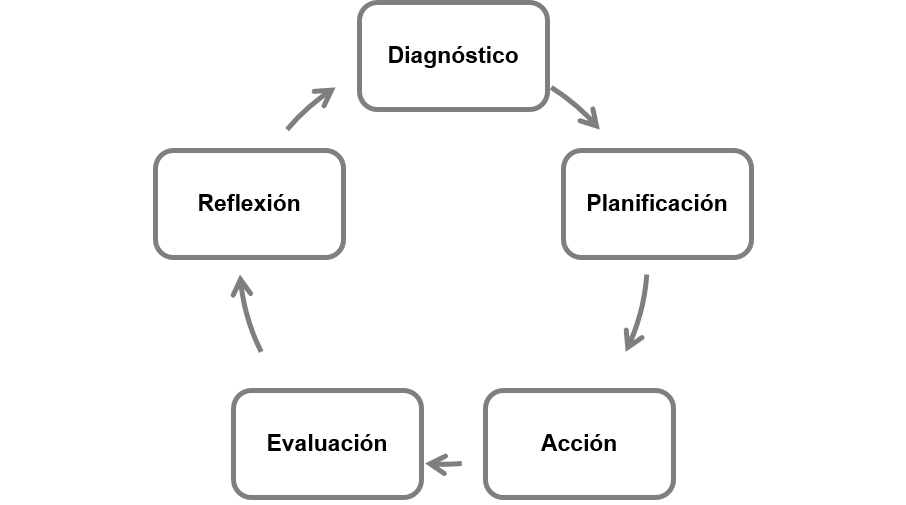
\includegraphics[scale=0.77]{img/investigacion-accion.png}
			\caption{\textbf{Figura 1.} \textit{Car\'{a}cter c\'{i}clico de la Investigaci\'{o}n-Acci\'{o}n} (Fuente: Baskerville, 1999).}
	\end{figure}
\FloatBarrier %you shall not pass table!!

	\begin{itemize}
		\item \textbf{Fase de diagn\'{o}stico:} se realiza el proceso de identificaci\'{o}n de los problemas primarios de la investigaci\'{o}n.
		\item \textbf{Fase de planificaci\'{o}n:} se especifican las acciones que se llevaran a cabo para solucionar los problemas primarios.
		\item \textbf{Fase de acci\'{o}n:} se ejecutan las acciones planificadas en la fase anterior.
		\item \textbf{Fase de evaluaci\'{o}n u observaci\'{o}n:} se efect\'{u}a una evaluaci\'{o}n de los resultados obtenidos, para observar, conocer y documentar los efectos de las acciones que fueron realizadas.
		\item \textbf{Fase de reflexi\'{o}n:} se toman los conocimientos adquiridos en la investigaci\'{o}n-acci\'{o}n. Si las acciones ejecutadas no fueron exitosas, los conocimientos pueden proporcionar la base para el diagn\'{o}stico de un nuevo ciclo de investigaci\'{o}n-acci\'{o}n.
	\end{itemize}

En la Tabla 2 se muestran las actividades de la presente investigaci\'{o}n, haciendo correspondencia a cada una de las fases de la Investigaci\'{o}n-Acci\'{o}n descritas por \cite{Baskerville}.

\FloatBarrier %you shall not pass table!!
\vline
	\begin{table}[htb]
		\small
		\caption{\textbf{Tabla 2.} \textit{Actividades del proyecto seg\'{u}n la Investigaci\'{o}n-Acci\'{o}n} (Fuente: Elaboraci\'{o}n propia).}
		\centering
		\setlength{\extrarowheight}{5pt}
		\begin{tabulary}{15cm}{|c|L|}
			\hline
			\thead{\textbf{\small{Fase}}} & \thead{\textbf{\small{Actividades}}}\\ \hline
			\textbf{Diagn\'{o}stico} & Identificar los problemas y limitaciones que presenta el HunterLab Universal Software.\\ \hline
			\textbf{Planificaci\'{o}n} & Seleccionar la metodolog\'{i}a de desarrollo, determinar los requisitos del software y realizar un plan de trabajo.
\\ \hline
			\textbf{Acci\'{o}n} & Desarrollar el software, tomando en cuenta los requisitos identificados previamente, los lineamientos de dise\~{n}o y de calidad del software.\\ \hline
			\textbf{Evaluaci\'{o}n} & Realizar las pruebas de funcionalidad e interfaz gr\'{a}fica de usuario del nuevo software.\\ \hline
			\textbf{Reflexi\'{o}n} & Presentar los resultados y los an\'{a}lisis de las pruebas realizadas.\\ \hline
		\end{tabulary}
	\end{table}
\FloatBarrier %you shall not pass table!!

	\section{Metodolog\'{i}a de Desarrollo de Software}
Para que el desarrollo del nuevo software cumpliera con los objetivos propuestos la presente investigaci\'{o}n, y tomando en cuenta los lineamientos planteados por la ingenier\'{i}a del software, se realiz\'{o} una revisi\'{o}n del enfoque que deber\'{i}a tener la metodolog\'{i}a de desarrollo a utilizar.

Seg\'{u}n \cite{Sommerville}, en los a\~{n}os 80 y a principios de los 90, exist\'{i}a una opini\'{o}n general de que la mejor forma de obtener un mejor software era a trav\'{e}s de una planificaci\'{o}n cuidadosa del proyecto, una garant\'{i}a de calidad formalizada, la utilizaci\'{o}n de m\'{e}todos de an\'{a}lisis y dise\~{n}o soportados por herramientas \textit{CASE}, y por medio de procesos de desarrollo de software controlados y rigurosos. El software que segu\'{i}a lo mencionado previamente, era desarrollado por grandes equipos que a veces trabajaban para compa\~{n}\'{i}as diferentes, que a menudo estaban dispersos geogr\'{a}ficamente y trabajaban en el software durante largos periodos de tiempo.

Ahora bien, debido a que no se dispuso de un equipo grande para el desarrollo del nuevo software, y a que no se iba a trabajar en este durante un largo periodo de tiempo, se eligi\'{o} la utilizaci\'{o}n de una metodolog\'{i}a de desarrollo de enfoque \'{a}gil. Acorde con \cite{Sommerville}, los m\'{e}todos \'{a}giles dependen de un enfoque iterativo para la especificaci\'{o}n, desarrollo y entrega del software, y est\'{a}n pensados para entregar software funcional de forma r\'{a}pida a los clientes, quienes pueden entonces proponer que se incluyan en iteraciones posteriores del software nuevos requerimientos o cambios en los mismos. Si bien los m\'{e}todos \'{a}giles proponen procesos diferentes para el desarrollo y entrega incrementales de software, comparten unos principios en com\'{u}n, los cuales son ilustrados en la Tabla 3.

\FloatBarrier %you shall not pass table!!
\vline
	\begin{table}[htb]
		\small
		\caption{\textbf{Tabla 3.} \textit{Principios de los m\'{e}todos \'{a}giles} (Fuente: Sommerville, 2005).}
		\centering
		\setlength{\extrarowheight}{5pt}
		\begin{tabulary}{15cm}{|c|L|}
			\hline
			\thead{\textbf{\small{Principio}}} & \thead{\textbf{\small{Descripci\'{o}n}}}\\ \hline
			\textbf{Participaci\'{o}n del cliente} & Los clientes deben estar fuertemente implicados en todo el proceso de desarrollo.\\ \hline
			\textbf{Entrega incremental} & El software se desarrolla en incrementos, en los que el cliente especifica los requerimientos a incluir en cada incremento.\\ \hline
			\textbf{Personas, no procesos} & Se deben reconocer y explotar las habilidades del equipo de desarrollo. A este se les debe dejar desarrollar su propia forma de trabajar, sin procesos formales.\\ \hline
			\textbf{Aceptar el cambio} & Se debe contar con que los requerimientos del software cambian, por lo que el software se dise\~{n}a para dar cabida a estos cambios.\\ \hline
			\textbf{Mantener la simplicidad} & Se debe centrar la simplicidad tanto en el software a desarrollar como en el proceso de desarrollo. Donde sea posible, se trabaja activamente para eliminar la complejidad del software.\\ \hline
		\end{tabulary}
	\end{table}
\FloatBarrier %you shall not pass table!!

		\subsection{Metodolog\'{i}a SCRUM}
De acuerdo con \cite{Schwaber&Sutherland}, esta metodolog\'{i}a \'{a}gil es un marco de trabajo de procesos, que ha sido utilizado para gestionar el desarrollo de productos complejos desde principios de los a\~{n}os 90. SCRUM muestra la eficacia relativa de las pr\'{a}cticas de gesti\'{o}n de productos y las pr\'{a}cticas de desarrollo.

La estructura de desarrollo de SCRUM se basa en ciclos de trabajo llamados \textit{sprints}. Estos \textit{sprints} son iteraciones de una a cuatro semanas que suceden una detr\'{a}s de la otra, con una duraci\'{o}n fija y con fechas de culminaci\'{o}n previamente establecidas. Se seleccionan los requerimientos que se van a desarrollar de una lista priorizada. Todos los d\'{i}as el equipo se re\'{u}ne, y al final del \textit{sprint} el equipo revisa el mismo con los \textit{stakeholders}.

\cite{Hundermark} explica de forma precisa los roles que conforman el equipo de desarrollo de SCRUM:

		\subsubsection{Los Roles}
			
			\begin{itemize}
				
				\item \textbf{Due\~{n}o del producto \textit{(Product Owner)}:} su responsabilidad es optimizar el retorno de la inversi\'{o}n, asegurando que el equipo SCRUM este ocupado en entregar las caracter\'{i}sticas m\'{a}s valiosas del producto. Su trabajo principal es concentrarse en la efectividad, esto es construir el producto correcto para sus clientes.
				
				\item \textbf{Equipo de desarrollo:} es una colecci\'{o}n de personas responsables por entregar incrementos de la funcionalidad del producto al final de cada \textit{sprint}. El trabajo principal de este equipo es concentrarse en la eficiencia, esto es construir el producto correcto para su \textit{Product Owner} y sus usuarios.
				
				\item \textbf{Maestro SCRUM \textit{(SCRUM Master)}:} gestiona todos los aspectos del proceso del equipo SCRUM. Su trabajo principal es concentrarse en el progreso continuo del equipo, acortando los ciclos de retroalimentaci\'{o}n mediante los cuales aprende.
				
			\end{itemize}
			
		\subsubsection{Las Reuniones}
			Como es sabido, el \textit{sprint} marca cada una de las iteraciones dentro del ciclo de desarrollo de SCRUM. Por otra parte, la planificaci\'{o}n, la continua revisi\'{o}n y la retrospectiva definen el inicio y el final del \textit{sprint}. Las reuniones que ocurren en cada \textit{sprint} son las siguientes:
			
			\begin{itemize}
				\item \textbf{Reuni\'{o}n de planificaci\'{o}n del \textit{sprint}: }
				esta reuni\'{o}n marca el inicio de cada \textit{sprint}. Su prop\'{o}sito para el equipo SCRUM es planear el trabajo que van a realizar durante el \textit{sprint} actual.
				
				\item \textbf{Reuni\'{o}n diaria del \textit{sprint}: }
				el equipo de desarrollo se reune para comunicar y sincronizar su trabajo, para luego crear un plan para las siguientes 24 horas. Esta colaboraci\'{o}n es esencial para asegurar el progreso continuo y evadir cualquier obstrucci\'{o}n de trabajo.
				
				\item \textbf{Reuni\'{o}n de revisi\'{o}n del \textit{sprint}: }
				su prop\'{o}sito primario es el de inspeccionar lo que el equipo de desarrollo ha entregado y obtener una retroalimentaci\'{o}n de los participantes en la reuni\'{o}n, para adaptar el plan para el \textit{sprint} subsiguiente. Esta reuni\'{o}n est\'{a} abierta para todo el personal dentro de la organizaci\'{o}n.
				
				\item \textbf{Reuni\'{o}n de retrospectiva: }
				es la reuni\'{o}n final del \textit{sprint}, la cual nunca es omitida, sin importar lo que haya ocurrido en dicho \textit{sprint}. Mientras que la reuni\'{o}n de revisi\'{o}n del \textit{sprint} est\'{a} enfocada en el producto, esta reuni\'{o}n est\'{a} enfocada en el proceso, es decir, la forma en la que el equipo SCRUM est\'{a} trabajando en conjunto, incluyendo sus habilidades t\'{e}cnicas, las pr\'{a}cticas de desarrollo del software y las herramientas que est\'{a}n usando. Esta reuni\'{o}n se limita a los miembros del equipo SCRUM.
				
			\end{itemize}
			
		\subsubsection{Los Artefactos}
			
			\begin{itemize}
				\item \textbf{Pila del producto \textit{(product backlog)}: }
					es una lista de \'{i}tems de trabajo descritos en un nivel funcional, que necesitan ser realizados a lo largo del tiempo. Los requerimientos son emergentes, lo que significa que no se puede saber por adelantado todos los detalles acerca de qu\'{e} se quiere en el producto. Por esta raz\'{o}n este artefacto es un documento din\'{a}mico, que requiere un refinamiento constante para mantenerlo actual y \'{u}til.
				
				\item \textbf{Pila del \textit{sprint} \textit{(sprint backlog)}: }
				esta pila es visualizada por el equipo de desarrollo en un \textit{task board}, que es la representaci\'{o}n f\'{i}sica de la lista de trabajo que se ha resumido para realizar durante el \textit{sprint} actual. Este artefacto le dice al equipo SCRUM y a todos los dem\'{a}s qu\'{e} trabajo tienen planeado hacer en el \textit{sprint}, y su estado actual.
				
				\item \textbf{Incremento: }
				es la suma de todos los \'{i}tems de la pila del producto que cumplen con la definici\'{o}n de terminado al final del \textit{sprint}. El equipo de desarrollo presentar\'{a} este en la revisi\'{o}n del \textit{sprint}, y el \textit{Product Owner} determinar\'{a} cuando liberar este incremento.
				
			\end{itemize}
			
En esta metodolog\'{i}a se pueden emplear varias t\'{e}cnicas y procesos. Dicho lo anterior, adicionalmente a la utilizaci\'{o}n de SCRUM, se incluyeron algunos artefactos de la metodolog\'{i}a RUP (Rational Unified Process) descrita por \cite{Kroll&Kruchten}, para as\'{i} generar suficiente documentaci\'{o}n durante el dise\~{n}o y el desarrollo del nuevo software. La configuraci\'{o}n de la metodolog\'{i}a SCRUM utlizada, en conjunto con los artefactos elegidos de la metodolog\'{i}a RUP, es la ilustrada en la Tabla 5.

\FloatBarrier %you shall not pass table!!
		\begin{table}[htb]
			\small
			\caption{\textbf{Tabla 5.} \textit{Configuraci\'{o}n de los artefactos a utilizar de SCRUM y RUP} (Fuente: Elaboraci\'{o}n propia).}
			\centering
			\setlength{\extrarowheight}{5pt}
			\begin{tabulary}{15cm}{|J|}
				\hline
				\thead{\textbf{\small{Artefactos SCRUM}}}\\ \hline
				\textbf{Pila del producto: }lista din\'{a}mica de las cosas que se deben hacer, sin especificar c\'{o}mo se deben hacer.\\ \hline
				\textbf{Pila del \textit{sprint}:} recopilaci\'{o}n resumida de los \'{i}tems de la pila del producto, en donde se dividen los \'{i}tems en tareas peque\~{n}as que no demanden una labor superior a una jornada de trabajo.\\ \hline
				\textbf{Incremento: }el producto final de cada \textit{sprint}. El mismo debe asemejarse a un software funcionando, permitiendo implementarse operativamente sin restricciones en un ambiente productivo.\\ \hline
				\thead{\textbf{\small{Artefactos RUP}}}\\ \hline
				\textbf{Documento de visi\'{o}n: }define el alcance en alto nivel y prop\'{o}sito del producto.\\
\hline
				\textbf{Glosario: }documento que define la terminolog\'{i}a empleada en los artefactos.\\ \hline
				\textbf{Documento de requerimientos no funcionales: }describe los requerimientos que tienen un impacto significativo en la arquitectura y en la satisfacci\'{o}n del usuario.\\ \hline
		\textbf{Diagrama de casos de uso: }muestra los procesos del negocio que son proporcionados para los actores del negocio.\\ \hline
			\end{tabulary}
		\end{table}
\FloatBarrier %you shall not pass table!!